\chapter{Il modello di Ising}

L'Hamiltoniana del modello di Ising è data da
%---
\be
\Ham = -J\sum_{\langle i,j\rangle}\sigma_{i}\sigma_{j} - h\sum_{i}\sigma_{i}
\ee
%---
in cui:
\begin{itemize}
\item gli indici $i,j$ sono interi che etichettano i siti di un reticolo;
\item $\langle i,j\rangle$ significa somma su $i$ e $j$ primi vicini;
\item $\sigma_{i}$ è una variabile di spin, il cui valore può essere $\pm 1$;
\item $J$ è il parametro di interazione, e se $J > 0$ spin primi vicini tendono
a stare allineati (la configurazione è energeticamente favorita);
\item $h$ è un eventuale campo magnetico esterno.
\end{itemize}

Questo modello è un ottimo punto di partenza per studiare il comportamento
critico (cioè alla transizione) di materiali ferromagnetici. Tali materiali
mostrano una magnetizzazione spontanea se la temperatura d'equilibrio è
inferiore a una temperatura critica $T_{c}$, detta {\em temperatura di Curie}.

Nel linguaggio del nostro modello la magnetizzazione totale $M$ è data da
%---
\be
M = \langle \sum_{i}\sigma_{i}\rangle
\ee
%---
Se il sistema è composto da $N$ spin possiamo definire una densità di
magnetizzazione $m = M/N$, che continueremo a chiamare magnetizzazione. Il
valore d'aspettazione è definito nell'ambito del formalismo canonico:
%---
\be
M =
\frac{1}{Q}\sum_{[\sigma]}\left(\sum_{i}\sigma_{i}\right)e^{-\beta\Ham[\sigma]}
\ee
%---
in cui
%---
\be
\sum_{[\sigma]} = \sum_{\sigma_{1} = \pm 1}\sum_{\sigma_{2} = \pm
1}\cdots\sum_{\sigma_{N} = \pm 1}
\ee
%---
Si vede subito che
%---
\be
M = \frac{1}{\beta}\frac{\partial \ln Q}{\partial h}
\ee
%---
e $Q$ è ovviamente la funzione di partizione del sistema:
%---
\be
Q = \sum_{[\sigma]}e^{-\beta\Ham[\sigma]}
\ee
%---
Pur nella sua semplicità, il modello di Ising è stato risolto in maniera esatta
solo in dimensione $D = 1$ e in dimensione $D = 2$ ma solamente per $h=0$.

\section{Il modello in una dimensione}

In $D = 1$ il modello di Ising può essere risolto in molti modi. Ci limiteremo a illustrare i due più interessanti: l'espansione esatta ad alta temperatura e il
metodo della matrice di trasferimento.

\subsection{Espansione ad alta temperatura}

Poniamo il campo magnetico $h=0$ e imponiamo condizioni periodiche al contorno:
$\sigma_{N+1} = \sigma_{1}$. Possiamo scrivere
\be
\Ham = -J\sum_{i=1}^N \sigma_{i}\sigma_{i+1}
\ee
Utilizziamo l'identità
\bea
\exp(\beta J \sigma_i \sigma_{i+i}) &=&
\cosh(\beta J) + \sigma_i \sigma_{i+i} \sinh(\beta J) \nonumber \\
&=& \cosh(\beta J) \left[ 1 + \sigma_i \sigma_{i+i} t \right]
\eea
con $t \equiv \tanh(\beta J)$. Per la funzione di partizione possiamo dunque
scrivere
\be
Q = \left[ \cosh(\beta J) \right]^N \sum_{[\sigma]} \prod_{i=1}^N
(1 + \sigma_i \sigma_{i+i} t)
\ee
Scrivendo esplicitamente la produttoria,
\be
Q = \left[ \cosh(\beta J) \right]^N \sum_{[\sigma]} (1+\sigma_1\sigma_2
t)(1+\sigma_2\sigma_3 t) \cdots (1+\sigma_N\sigma_1 t)
\ee
vediamo che possiamo riscrivere la produttoria stessa come una serie in potenze di $t$ (per questo è un'espansione ad alta temperatura, perché se $T\to\infty$ allora $t\to 0$):
\bea
Q &=& \left[ \cosh(\beta J) \right]^N \sum_{[\sigma]} 
[
1 + t(\sigma_1\sigma_2 + \sigma_2\sigma_3 + \cdots)  \nonumber\\
&& + t^2 (\sigma_1\sigma_3 + \sigma_1\sigma_2\sigma_3\sigma_4 + \cdots)
+ \cdots + t^N
]
\eea
Quando sommiamo su $\sigma_i = \pm 1$, tutti i termini che contengono $\sigma_i$ si annullano nella somma. Considerando che il numero totale di configurazioni è pari a $2^N$ otteniamo
\be
Q = \left[ 2\cosh(\beta J) \right]^N (1 + t^N)
\ee
Poiché $t$ è sempre minore di $1$, nel limite termodinamico il termine $t^N$ scompare. Otteniamo quindi, per l'energia libera,
\be
A = -kT\ln Q = -Nkt \ln[2\cosh(J/kT)]
\ee

\subsection{La matrice di trasferimento}

Con condizioni periodiche al contorno e $h \ne 0$ possiamo riscrivere
l'Hamiltoniana in maniera simmetrica:
%---
\be
\Ham = -J\sum_{i}\sigma_{i}\sigma_{i+1} -
\frac{h}{2}\sum_{i}(\sigma_{i}+\sigma_{i+1})
\ee
%---
Introducendo i vettori di stato $|\sigma_{i}\rangle$ e l'operatore $\hat{P}$,
con elementi di matrice uguali a
%---
\be
\langle\sigma_{i}| \hat{P} |\sigma_{i+1}\rangle =
\exp\left\{\beta[J\sigma_{i}\sigma_{i+1} + h(\sigma_{i}+\sigma_{i+1})/2]
\right\}
\ee
%---
possiamo riscrivere la funzione di partizione in questo modo:
%---
\be
Q = \sum_{\sigma_{1} = \pm 1}\sum_{\sigma_{2} = \pm 1}\cdots\sum_{\sigma_{N} =
\pm 1}
\langle\sigma_{1}| \hat{P} |\sigma_{2}\rangle\langle\sigma_{2}| \hat{P}
|\sigma_{3}\rangle\cdots\langle\sigma_{N}| \hat{P} |\sigma_{1}\rangle
\ee
%---
Poiché vale la relazione di completezza
%---
\be
\sum_{\sigma_{i}=\pm 1}|\sigma_{i}\rangle\langle\sigma_{i}| = 1\quad \forall i
\ee
%---
otteniamo facilmente
%---
\be
Q = \sum_{\sigma_{1}=\pm 1}\langle\sigma_{1}| \hat{P}^{N} |\sigma_{1}\rangle =
\mbox{Tr}(\hat{P}^{N}) = \lambda_{1}^{N} + \lambda_{2}^{N}
\ee
%---
in cui $\lambda_{1}$ e $\lambda_{2}$ sono gli autovalori della matrice
%---
%\myformula{-}{
%P = \startmatrix[left={\left(\,},right={\,\right)}]
%\NC e^{\beta(J+h)} \NC e^{-\beta J}    \NR
%\NC e^{-\beta J}   \NC e^{\beta(J-h)}  \NR
%\stopmatrix
%}
%---
L'equazione quadratica che li definisce è:
%---
\be
\lambda^{2} - \lambda e^{\beta J}(e^{\beta h} + e^{-\beta h}) + e^{2\beta J} - e^{-2\beta J}= 0
\ee
%---
e con un po' di manipolazione algebrica troviamo
%---
\be
\lambda = e^{\beta J} \cosh(\beta h) \pm \sqrt{e^{-2\beta J} + e^{2\beta
J}\sinh^{2}(\beta h)}
\ee
%---
Poiché $\lambda_{2} < \lambda_{1}$ possiamo scrivere 
%---
\be
Q = \lambda_{1}^{N}[1+(\lambda_{2}/\lambda_{1})^{N}]
\ee
%---
e quindi nel limite termodinamico ($N\to\infty$) conta solo l'autovalore più
grande. Quindi per l'energia libera di Von Helmholtz otteniamo
%---
\be
A = -\frac{1}{\beta}\ln Q \simeq -\frac{N}{\beta}\ln\lambda_{1}
\ee
%---
e per la magnetizzazione otteniamo
%---
\be
M = -\left(\frac{\partial A}{\partial h}\right)_{T} = \frac{N\sinh(\beta h)}
{\sqrt{e^{-4\beta J}+\sinh^{2}(\beta h)}}
\ee
%---
Vediamo subito che se $h=0$ la magnetizzazione è nulla per tutte le temperature
maggiori di zero. Questo significa che in una dimensione il modello di Ising non presenta la transizione di fase ferromagnetica.

Se $J=0$ ritroviamo il risultato paramagnetico, ossia
%---
\be
M = N\tanh(\beta h)
\ee
%---

\section{Approssimazione di campo medio}

Il conto esatto in due dimensioni risulta abbastanza complicato. Come prima
approssimazione, valida in dimensione $D$ qualsiasi, partiamo dal cosiddetto
{\em campo medio}, un approccio variazionale basato sulla minimizzazione
dell'energia libera. Ciò che si minimizza, però, non è la {\em vera} energia
libera, ma un funzionale ``energia libera'' che deriva da una distribuzione di
probabilità fattorizzata. Scriviamo cioè
%---
\be
\rho_{\mbox{mf}}[\sigma] = \prod_{i}\rho_{i}(\sigma_{i})
\ee
%---
in cui
%---
\be
\rho_{i}(\sigma) = \frac{1+m_{i}}{2}\delta_{\sigma,1} +
\frac{1-m_{i}}{2}\delta_{\sigma,-1}
\ee
%---
in cui $m_{i}$ è il parametro su cui effettueremo la minimizzazione. Il suffisso``mf'' sta per {\em mean field}, ossia campo medio. La $\rho$ di campo medio è
normalizzata a 1:
%---
\be
\sum_{\sigma_{i}=\pm 1}\rho_{i}(\sigma_{i}) = \frac{1+m_{i}}{2} +
\frac{1-m_{i}}{2} = 1
\ee
%---
e quindi
%---
\be
Q_{\mbox{mf}} = \sum_{[\sigma]}\rho_{\mbox{mf}} = 1
\ee
%---
e otteniamo subito
%---
\be
\langle A[\sigma_{i}] \rangle_{\mbox{mf}} = \frac{1+m_{i}}{2}A(1) +
\frac{1-m_{i}}{2}A(-1)
\ee
%---
In particolare l'ultima equazione implica
%---
\be
\langle \sigma_{i} \rangle_{\mbox{mf}} = \frac{1+m_{i}}{2} - \frac{1-m_{i}}{2}A
= m_{i}
\ee
%---
e quindi $m_{i}$ è proprio la magnetizzazione locale nel punto $i$. Nel seguito
per semplicità ometteremo il sottoscritto ``mf''. La fattorizzazione della
$\rho$ implica
%---
\be
\aspetta{AB} = \aspetta{A}\aspetta{B}
\ee
%---
in modo tale che possiamo immediatamente scrivere
%---
\be
U = \aspetta{\Ham} = -J\sum_{\langle i,j\rangle}m_{i}m_{j} - h\sum_{i}m_{i}
\ee
%---
Per l'entropia otteniamo invece
%---
\be
S = -\aspetta{\ln\rho} = -\sum_{i}\aspetta{\ln\rho_{i}} = -\sum_{i}s_{i}
\ee
%---
in cui
%---
\be
s_{i} = \frac{1+m_{i}}{2}\ln\left(\frac{1+m_{i}}{2}\right) +
\frac{1-m_{i}}{2}\ln\left(\frac{1-m_{i}}{2}\right)
\ee
%---
Definiamo un funzionale $\Phi$ tale che se $\rho$ fosse la giusta distribuzione
di Boltzmann allora $\Phi$ sarebbe l'energia libera:
%---
\be
\Phi = U - \frac{1}{\beta}S = -J\sum_{\langle i,j\rangle}m_{i}m_{j} -
h\sum_{i}m_{i}-\frac{1}{\beta}\sum_{i}s_{i}
\ee
%---
in cui abbiamo posto $k=1$, e quindi la temperatura ha le stesse dimensioni
fisiche di un'energia. Imponiamo ora la condizione di estremizzazione, ossia
deriviamo $\Phi$ rispetto a $m_{i}$ e imponiamo che la derivata sia nulla. Per
semplificare i conti scriviamo
%---
\be
-J\sum_{\langle i,j\rangle}m_{i}m_{j} \equiv -\sum_{i,j}J_{ij}m_{i}m_{j}
\ee
%---
in cui $J_{ij}$ è una matrice i cui elementi valgono $J$ se $i$ e $j$ sono primivicini e $0$ altrimenti. Otteniamo
%---
\be
\dpar{\Phi}{m_{i}} = -\sum_{j}J_{ij}m_{j} - h +
\frac{1}{\beta}\mbox{arctanh}(m_{i})
\ee
%---
nella quale è stata usata l'identità
%---
\be
\ln\sqrt{\frac{1+m}{1-m}} = \mbox{arctanh}(m)
\ee
%---
Troviamo quindi l'equazione fondamentale di campo medio:
%---
\be
m_{i} = \tanh\left[\beta\left(\sum_{j}J_{ij}m_{j} + h\right)\right]
\ee
%---

\subsection{Un modo alternativo}

Possiamo ricavare l'equazione di campo medio partendo da un'equazione esatta.
Scriviamo
%---
\be
m_{i} = \aspetta{\sigma_{i}} =
\frac{1}{Q}\sum_{[\sigma]}\sigma_{i}e^{-\beta\Ham}
\ee
%---
(in cui ora il valore d'aspettazione è il ``vero'' valore d'aspettazione, non
quello di campo medio). Notiamo che possiamo scrivere
%---
\be
\Ham = \bar{\Ham} + \Ham_{i}
\ee
%---
nella quale
%---
\be
\Ham_{i} = \sum_{j} J_{ij}\sigma_{i}\sigma_{j} - h\sigma_{i}
\ee
%---
e $\bar{\Ham}$ contiene tutti gli altri termini che non coinvolgono
$\sigma_{i}$. Il valore d'aspettazione di $\sigma_{i}$ diventa quindi
%---
\be
m_{i} =
\frac{1}{Q}\sum_{[\sigma]}'\left(\sum_{\sigma_{i}=\pm1}\sigma_{i}e^{-\beta\Ham_{i}}\right)e^{-\beta\bar{\Ham}}
\ee
%---
in cui l'apice sulla prima sommatoria significa che stiamo escludendo la somma
su $\sigma_{i}$, che è scritta esplicitamente dopo. Ora possiamo moltiplicare e
dividere per la stessa quantità, ossia $\sum_{\sigma_{i}}e^{-\beta\Ham_{i}}$, e
otteniamo
%---
\be
m_{i} =
\frac{1}{Q}\sum_{[\sigma]}e^{-\beta\Ham}\left(\frac{\sum_{\sigma_{i}}\sigma_{i}e^{-\beta\Ham_{i}}}{\sum_{\sigma_{i}}e^{-\beta\Ham_{i}}}\right)
= \aspetta{\tanh\left[\beta\left(\sum_{j}J_{ij}\sigma_{j} + h\right)\right]}
\ee
%---
Se ora assumiamo che la distribuzione di probabilità sia fattorizzata, possiamo
scambiare il valore d'aspettazione della tangente iperbolica con la tangente
iperbolica del valore d'aspettazione; questo fatto è facilmente comprensibile
pensando alla tangente iperbolica come al suo sviluppo in serie di potenze e
considerando che per una distribuzione di probabilità fattorizzata, come abbiamonotato in precedenza, vale l'identità:
%---
\be
\aspetta{x^{n}} = \aspetta{x}^{n}
\ee
%---
Otteniamo quindi di nuovo l'equazione fondamentale di campo medio.

\subsection{Soluzioni dell'equazione di campo medio}

In questa sezione poniamo per semplicità $J=1$ (ossia misuriamo le energie e le
temperature in unità di $J$). Inoltre se $h$ è costante anche la magnetizzazionelocale sarà costante, ossia
%---
\be
m_{i} = m\quad\quad\forall i
\ee
%---
Abbiamo dunque, considerando che $\sum_{j}J_{ij}m_{j} = 2Dm$, 
%---
\be
m = \tanh[\beta(2Dm + h)]
\ee
%---
Poniamoci ora nel caso $h=0$. In questo caso $m=0$ è sempre una soluzione
dell'equazione precedente, ma vogliamo sapere se si tratta di un minimo o di un
massimo. Occorre calcolare la derivata seconda di $\Phi$. Definendo
$\phi\equiv\Phi/N$, nella nuova notazione abbiamo
%---
\be
\label{eq:derprima}
\dpar{\phi}{m} = -2Dm+\frac{1}{2\beta}\ln\frac{1+m}{1-m}
\ee
%---
e quindi
%---
\be
\frac{\partial^{2}\phi}{\partial m^{2}} = -2D +
\frac{1}{\beta}\frac{1}{1-m^{2}}\ee
%---
Perché una soluzione $m$ che annulla la derivata prima di $\phi$ sia un minimo
occorre che
%---
\be
1-m^{2} < \frac{1}{2D\beta}
\ee
%---
%%%
\begin{figure}[!ht]
  \centering
  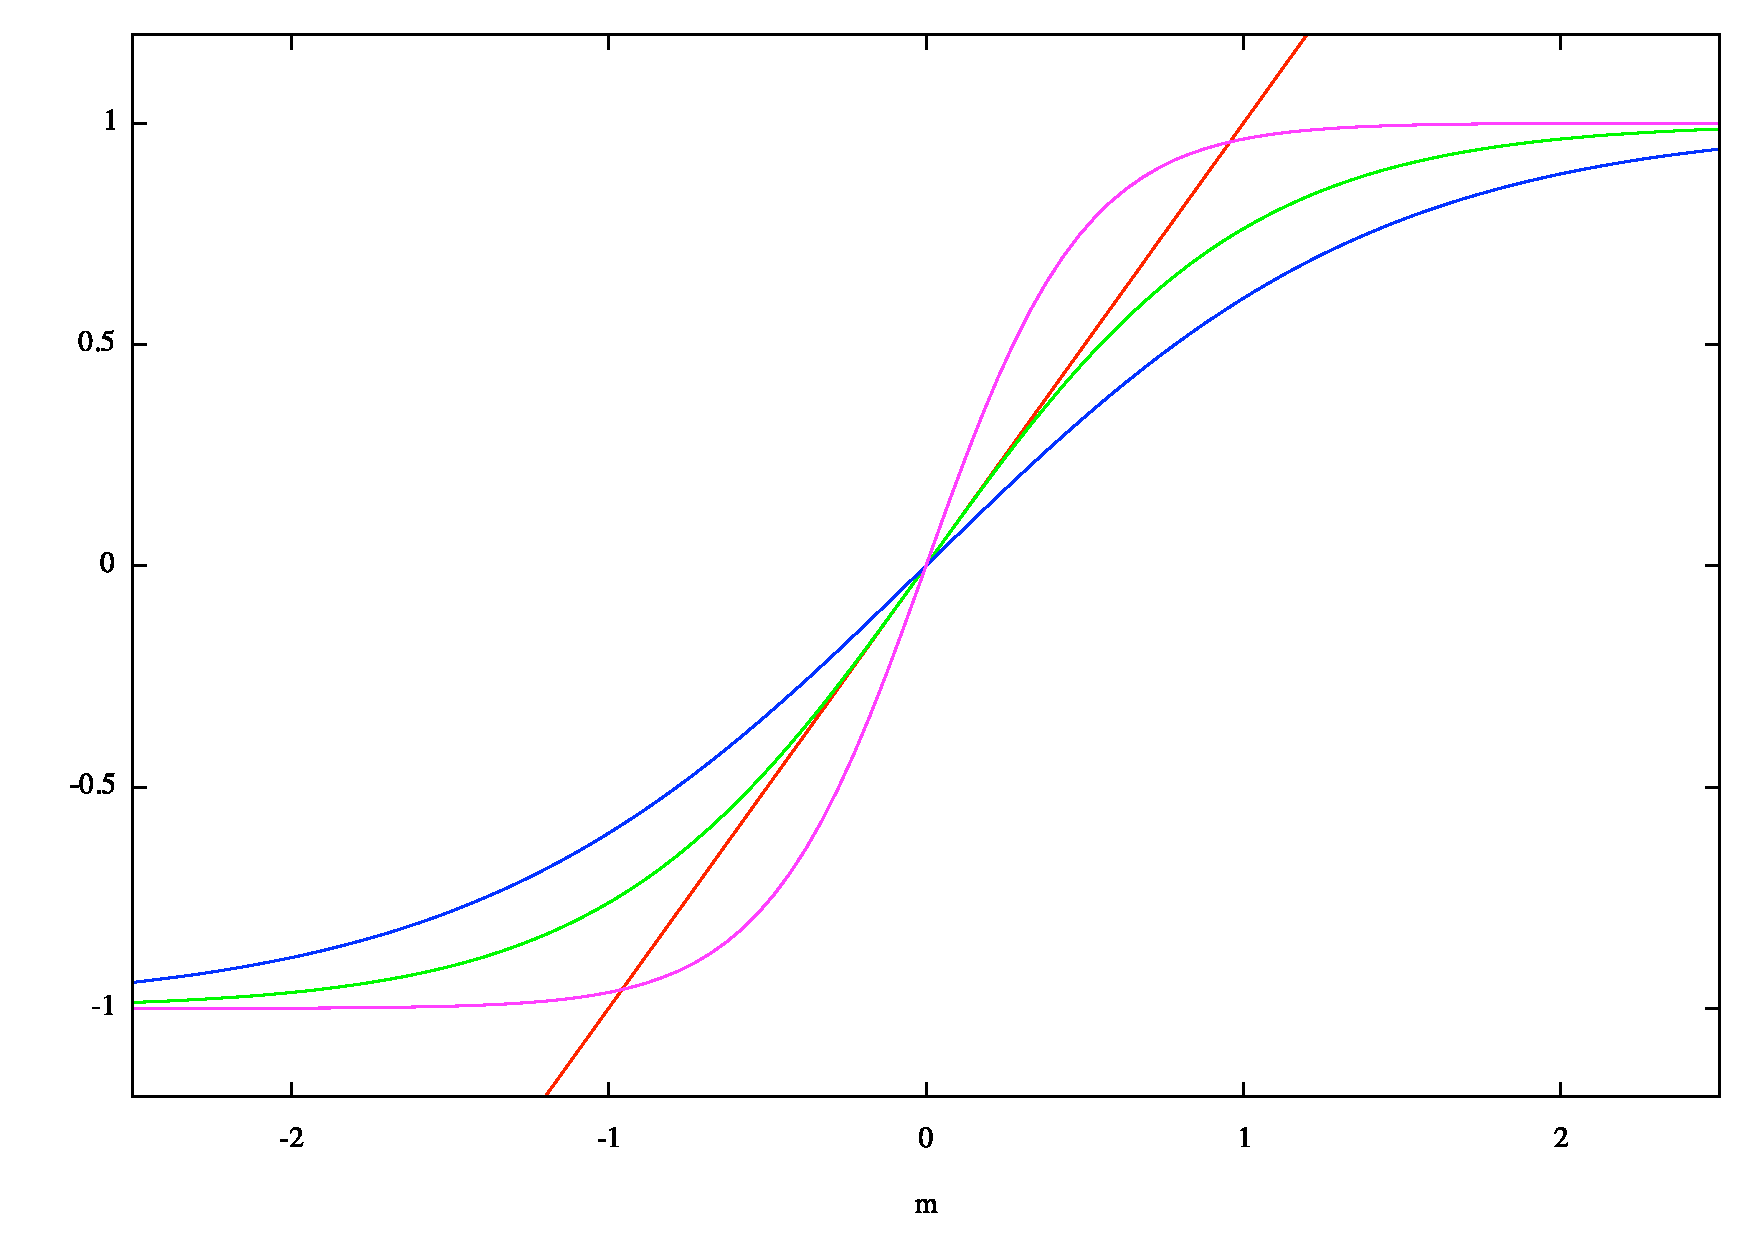
\includegraphics[width=0.75\textwidth]{mf.pdf}
\caption{Soluzione grafica dell'equazione di campo medio. La curva verde è la
tangente iperbolica calcolata per $\beta = \beta_{c}$.}
  \label{fig:mf}
\end{figure}
%%%

Ora, se $1/2D\beta > 1$ la derivata seconda di $\phi$ è sempre maggiore di zero,perché $m^{2}$ è sempre minore di $1$, quindi $m=0$ costituisce un minimo ed è
l'unica soluzione dell'equazione di campo medio. Invece se $1/2D\beta < 1$
allora $m=0$ è un massimo, e compaiono altre soluzioni. In Figura \ref{fig:mf}
c'è la visualizzazione grafica delle possibili soluzioni.

Appare dunque chiaro che $\beta_{c}\equiv 1/2D$ rappresenta un valore {\em
critico} di $\beta$; per valori di $\beta$ minori di $\beta_{c}$ (ovvero per
valori di $T > T_{c}$) il sistema non presenta magnetizzazione spontanea, che sisviluppa invece per valori della temperatura inferiori a quella critica.

Calcoliamo la magnetizzazione spontanea $m_{s}$ nel limite $T\to 0$, che
equivale a $\beta\to\infty$. In questo caso possiamo scrivere
%---
\be
\tanh(2D\beta m) \simeq 1 - 2e^{-4D\beta m}
\ee
%---
La magnetizzazione spontanea è dunque uguale a $1$ a meno di correzioni
esponenziali:
%---
\be
m_{s} \simeq \pm(1 - 2e^{-4D\beta})
\ee
%---
Invece per $T\to T_{c}^{-}$, ossia per $2D\beta\to 1^{+}$, sappiamo che la
magnetizzazione sarà vicina a zero, e questo ci permette di espandere la
tangente iperbolica:
%---
\be
m_{s} \simeq 2D\beta m_{s} - \frac{8D^{3}\beta^{3}m_{s}^{3}}{3}
\ee
%---
Vediamo però che $8D^{3}\beta^{3} = (\beta/\beta_{c})^{3}$, e dunque a
quest'ordine può essere trascurato: otteniamo quindi
%---
\be
m_{s}\propto(T_{c}-T)^{1/2}
\ee
%---
Per quel che riguarda la densità di energia interna, abbiamo $u = -Dm^{2}$.
Dunque per $T>T_{c}$ l'energia interna è nulla, mentre l'andamento critico al disotto di $T_{c}$ è chiaramente
%---
\be
u\propto(T_{c}-T)^{1}
\ee
%---
Il fatto che $u$ non sia discontinuo alla transizione implica che la transizionestessa non è del primo ordine (non c'è calore latente).
Se $T=T_{c}$ e $h\ne 0$ (ma piccolo in valore assoluto) abbiamo
%---
\be
m = \tanh(m+h) \simeq m + h - m^{3}/3
\ee
%---
(nella quale abbiamo trascurato un termine $O(h^{3})$), e otteniamo quindi
%---
\be
m \propto h^{1/3}
\ee
%---
Va notato che l'approssimazione di campo medio prevede una transizione di fase
anche in $D=1$, cosa che sappiamo essere falsa.

\subsection{Un modello esattamente risolubile}

La soluzione esatta del modello di Ising in $D=2$ e le soluzioni numeriche in
$D=3$ e in dimensioni superiori mostrano che l'approssimazione di campo medio
diventa sempre migliore al crescere di $D$. Questo risultato è intuitivamente
corretto: al crescere di $D$ cresce il numero di primi vicini di un determinato
spin (il numero di coordinazione di un reticolo semplicemente cubico è pari a
$2D$), e quindi è ragionevole supporre che l'approssimazione di campo medio, chesi basa proprio sul fatto che la magnetizzazione locale è data dal ``campo
medio'' dei primi vicini, migliori al crescere del numero di siti reticolari coni quali un dato spin interagisce direttamente.

Per rendere più concreta questa affermazione utilizziamo un modello esattamente
risolubile. L'Hamiltoniana è uguale a quella di Ising, ma ogni spin interagisce
con tutti gli altri spin del reticolo. Allo stesso tempo l'accoppiamento $J$
descresce con $N$, il numero di spin totali. Abbiamo dunque
%---
\be
e^{-\beta\Ham} = \exp\left(\frac{\beta}{2N}\sum_{i,j}\sigma_{i}\sigma_{j} +
\beta h\sum_{i}\sigma_{i} \right)
\ee
%---
in cui il fattore $2$ ci permette di sommare due volte su tutti gli spin. La
peculiarità di questo modello è che il fattore di Boltzmann può essere espresso
come un integrale gaussiano:
%---
\be
e^{-\beta\Ham} =
\left(\frac{N\beta}{2\pi}\right)^{1/2}\int_{-\infty}^{\infty}\de{\lambda}\,\exp\left(
-\frac{N\beta\lambda^{2}}{2} +\sum_{i}(\beta\lambda + \beta h)\sigma_{i}\right)
\ee
%---
e possiamo quindi scrivere
%---
\be
Q = \sum_{[\sigma]}e^{-\beta\Ham} =
\left(\frac{N\beta}{2\pi}\right)^{1/2}\int_{-\infty}^{\infty}\de{\lambda}\,\exp\left(-\frac{N\beta\lambda^{2}}{2}\right)
\sum_{[\sigma]}
\prod_{i}\exp\left((\beta\lambda + \beta h)\sigma_{i}\right)
\ee
%---
Invertendo la somma sulle configurazioni con la produttoria su tutti i siti,
otteniamo
%---
\be
Q =
\left(\frac{N\beta}{2\pi}\right)^{1/2}\int_{-\infty}^{\infty}\de{\lambda}\,\exp\left(-\frac{N\beta\lambda^{2}}{2}\right)\left\{
2\cosh[\beta(\lambda+h)]\right\}^{N}
\ee
%---
e in definitiva
%---
\be
Q =
\left(\frac{N\beta}{2\pi}\right)^{1/2}\int_{-\infty}^{\infty}\de{\lambda}\,e^{N\beta
B(\lambda)}
\ee
%---
in cui
%---
\be
B(\lambda) = -\frac{\lambda^{2}}{2} +
\frac{1}{\beta}\ln\{2\cosh[\beta(\lambda+h)]\}
\ee
%---
Il metodo dello {\em steepest descent} ci dice che
%---
\be
\lim_{N\to\infty} \frac{1}{N}\ln\left\{
\int_{-\infty}^{\infty}\de{x}\,e^{Ng(x)}\right\} = \max_{x}\{g(x)\} + O(N^{-1})
\ee
%---
e per la densità di energia libera otteniamo proprio
%---
\be
f = \frac{A}{N} = -\frac{1}{N\beta}\ln Q
\ee
%---
Dunque per calcolare $f$ nel limite termodinamico sarà sufficiente calcolare il
massimo della funzione $B(\lambda)$. Si ottiene facilmente che il valore di
$\lambda$ che massimizza la funzione $B(\lambda)$ soddisfa l'equazione
%---
\be
\bar{\lambda} = \tanh(\beta h +\beta\bar{\lambda})
\ee
%---
e ci chiediamo ora qual è il significato fisico di $\bar\lambda$. Calcoliamo la
magnetizzazione del sistema:
%---
\be
f = -\frac{B(\bar\lambda)}{\beta}\quad\quad m = -\dpar{f}{h}
\ee
%---
e si trova facilmente
%---
\be
m = \frac{1}{\beta}\dpar{B(\bar\lambda)}{h} = \tanh(\beta h
+\beta\bar{\lambda})\ee
%---
e dunque $\bar{\lambda} = m$. Quindi in questo caso l'equazione di campo medio
risolve esattamente il modello.
